\subsection{Esquema del servidor}

    El esquema de servidor se basa en el patrón \emph{MVC} (Modelo, Vista, Controlador) que provee \emph{CodeIgniter} con su framework.

    El modo de funcionar este patrón es el siguiente:

        \begin{itemize}
            \item Un usuario lanza una petición contra la siguiente url

                http://www.example.com/clientes/get\_cliente/1

            \item A través del modulo mod\_rewrite se redirige la petición al fichero \emph{index.php} de CodeIgniter, el cual se encarga de analizar la petición siguiendo el siguiente flujo de trabajo:

            \begin{figure}[H]
                \centering
                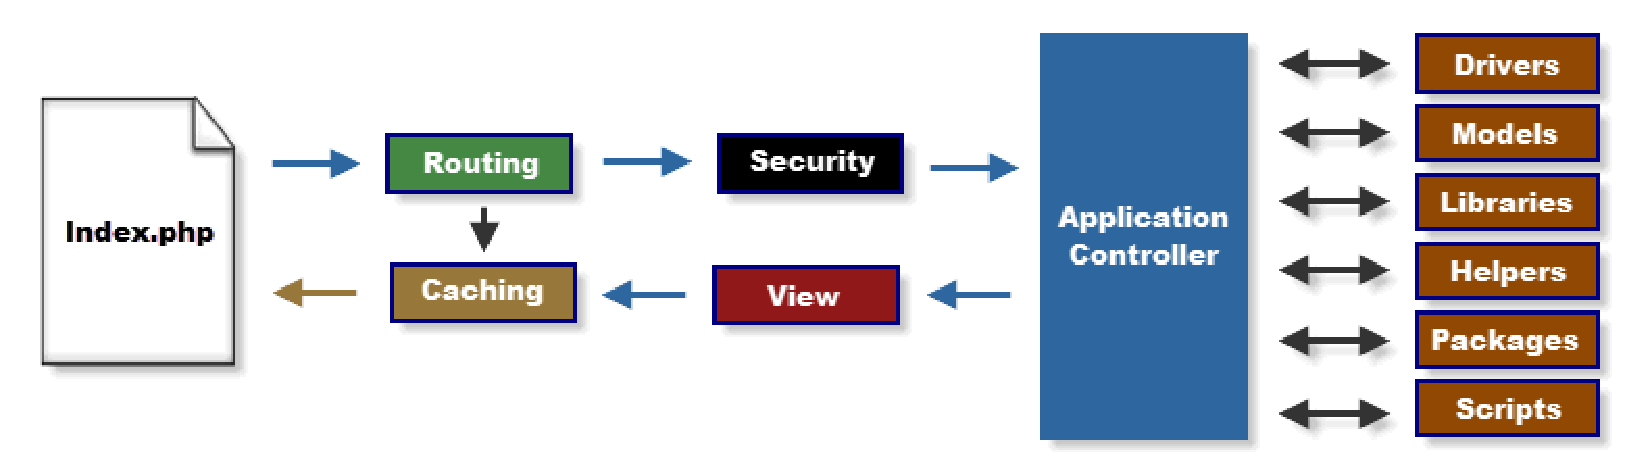
\includegraphics[keepaspectratio,width=0.9\textwidth]{flujo-trabajo-codeigniter.eps}
                \caption{Flujo de trabajo de CodeIgniter}\label{fig:flujo-trabajo-codeigniter}
            \end{figure}

            \item CodeIgniter descompone la URL en la siguiente estructura para conocer a que controlador tiene que pasar la petición, a que función llamar y qué parametros debe pasar.

                http://example.com/[controller-class]/[controller-method]/[arguments]

            Siendo para nuestro ejemplo los siguientes valores:

                \begin{itemize}
                    \item Controller class: clientes
                    \item Controller method: get\_cliente
                    \item Arguments: 1
                \end{itemize}
        \end{itemize}

    Los controladores son los encargados de procesar la petición, cargar tantas librerías, modelos... como necesiten para finalmente devolver un resultado.

    \subsubsection{Extendiendo el core de CodeIgniter}

    CodeIgniter al cargarse intenta buscar los sisguientes ficheros de sistema en la carpeta \emph{application/core}, esta funcionalidad permite sobreescribir algunas de las funcionalidades para ampliarlas.

    En el proyecto se han creado dos nuevos controladores para ampliar la funcionalidad del controlador por defecto de CodeIgniter:

    \begin{itemize}
        \item MY\_Controller

        Extiende de \emph{CI\_Controller} y se encarga de:

            \begin{itemize}
                \item Cargar la librería \emph{login\_auth} si no se están ejecutando los tests unitarios
                \item Ofrecer los siguientes métodos para renderizar la respuesta (\emph{\_renderJson}, \emph{\_renderXml}, \emph{\_renderToVar}, \emph{\_render})
            \end{itemize}

        \item MY\_Controller\_User

        Extiende de \emph{MY\_Controller} y únicamente se encarga de validar en el constructor que el usuario está logueado en el sistema, en caso de no estarlo, redirije a la Home pública.
    \end{itemize}

    \subsubsection{Esquema de controladores}

El esquema de controladores se pueden dividir en dos partes; aquellos que permiten el acceso a la web (la aplicación web los utiliza para renderizar la página) y controlan la sesión del usuario; y aquellos que funcionan como una API \emph{RESTful}, solamente devuelven objetos \emph{JSon}.

Controladores de acceso web

    \begin{itemize}
        \item home.php

            Se encarga de renderizar la parte pública de la web y controlar las acciones de registro de usuario, recordatorio de contraseña y acceso a la zona privada de usuario.

        \item tablon.php

            Se encarga de renderizar el esqueleto de la parte privada de usuario, de controlar que está logueado en el sistema y de permitir salir de su sesión.
    \end{itemize}

Controladores de API \emph{RESTful}

    \begin{itemize}
        \item fridge.php

            Se encarga de procesar las solicitudes para manejar los frigoríficos del usuario y los productos que contienen, así como sus compras.

        \item supermercado.php

            Se encarga de procesar las solicitudes para manejar los supermercados y los productos que contienen.

    \end{itemize}

    \subsubsection{Esquema de librerías}

La única restricción que se ha encontrado en CodeIgniter para hacer tests unitarios es que los controladores no se pueden cargar para hacerles pruebas unitarias. Por ello, toda la funcionalidad compleja se traslada a una librería específica la cual tiene sus tests unitarios.

De esta manera el controlador, no necesita de tests unitarios ya que actua como mediador entre el cliente y las librerías.

Se han implementado las siguientes librerías en el sistema:

    \begin{itemize}
        \item Login\_auth\_library.php
        \item My\_PHPMailer.php
        \item Fridge\_library.php
        \item Compra\_library.php
        \item Supermercado\_library.php
    \end{itemize}

    \subsubsection{Esquema de modelos}

        Antes de explicar el esquema de modelos es interesante comentar como funciona el acceso a base de datos.

        CodeIgniter utiliza una versión modificada del patrón \emph{Active Record Database}, lo que nos permite obtener, insertar y actualizar la base de datos con una mínima cantidad de código.

        Además, este patrón nos permite abstraernos del motor de base de datos, para cada motor de base de datos hay un adaptador que se encarga de generar las consultas SQL para funcionar contra él.

        A continuación se muestra una consulta generada con la \emph{Active Record class} de CodeIgniter:

        \begin{lstlisting}
private function get_total_compra($id_compra) {
    $this->db->select_sum('compra_producto.precio', 'total_compra');
    $this->db->from('compra_producto');
    $this->db->where('compra_producto.id_compra', $id_compra);

    $query = $this->db->get();

    if ($query->num_rows() === 1) {
        return $query->row()->total_compra;
    }
    return 0;
}
        \end{lstlisting}

        Una vez explicado el funcionamiento del acceso a Base de Datos, se expone a continuación el esquema de modelos utilizado:

        \begin{itemize}
            \item user\_model.php
            \item fridge\_model.php
            \item compra\_model.php
            \item supermercado\_model.php
        \end{itemize}